 \let\negmedspace\undefined
\let\negthickspace\undefined
\documentclass[journal]{IEEEtran}
\usepackage[a5paper, margin=10mm, onecolumn]{geometry}
%\usepackage{lmodern} % Ensure lmodern is loaded for pdflatex
\usepackage{tfrupee} % Include tfrupee package

\setlength{\headheight}{1cm} % Set the height of the header box
\setlength{\headsep}{0mm}     % Set the distance between the header box and the top of the text

\usepackage{gvv-book}
\usepackage{gvv}
\usepackage{cite}
\usepackage{amsmath,amssymb,amsfonts,amsthm}
\usepackage{algorithmic}
\usepackage{graphicx}
\usepackage{textcomp}
\usepackage{xcolor}
\usepackage{txfonts}
\usepackage{listings}
\usepackage{enumitem}
\usepackage{mathtools}
\usepackage{gensymb}
\usepackage{comment}
\usepackage[breaklinks=true]{hyperref}
\usepackage{tkz-euclide} 
\usepackage{listings}
% \usepackage{gvv}                                        
\def\inputGnumericTable{}                                 
\usepackage[latin1]{inputenc}                                
\usepackage{color}                                            
\usepackage{array}                                            
\usepackage{longtable}                                       
\usepackage{calc}                                             
\usepackage{multirow}                                         
\usepackage{hhline}                                           
\usepackage{ifthen}                                           
\usepackage{lscape}
\begin{document}

\bibliographystyle{IEEEtran}
\vspace{3cm}

\title{1.6.8}
\author{EE25BTECH11058 - Tangellapalli Mohana Krishna Sushma}
% \maketitle
% \newpage
% \bigskip
{\let\newpage\relax\maketitle}

\renewcommand{\thefigure}{\theenumi}
\renewcommand{\thetable}{\theenumi}
\setlength{\intextsep}{10pt} % Space between text and floats
\textbf{Question}:
If three points $\,(x, -1),\, \vec{(2, 1)}\, \text{and} \, \vec{(4, 5)}\,$ are collinear, find the value of $x$.


\bigskip

\textbf{Solution}:

\[
\begin{array}{|c|c|c|}
\hline
\textbf{Point} & \textbf{x} & \textbf{y} \\
\hline
A & x & -1 \\
B & 2 & 1 \\
C & 4 & 5 \\
\hline
\end{array}
\]


collinearity matrix can be expressed as


\begin{align*}
   \begin{myvec}{A-B & A-C\\}\end{myvec}=\begin{myvec}{x-2 & x-4\\-2 & -6\\}\end{myvec}
 \end{align*}


Changing the matrix in echelon form using row operation,

\[
\begin{myvec}{x-2 & x-4\\-2 & -6}\end{myvec}
\xrightarrow{R_2 \leftrightarrow R_1}
\begin{myvec}{-2 & -6\\x-2 & x-4}\end{myvec}
\xrightarrow{R_2 \rightarrow R_2 + ((x-2)/2)*R_1} 
\begin{myvec}{-2 & -6\\0 & -2x+2}\end{myvec}
\]



To make the following matrix Rank 1. (i.e., To prove collinearity)
Thus, we make the bottom row elements zero.



\begin{align*}
-2x + 2 = 0 \\
\Rightarrow x = 1 \\
\end{align*}

Hence, The value of x = 1.


\begin{figure}
    \centering
    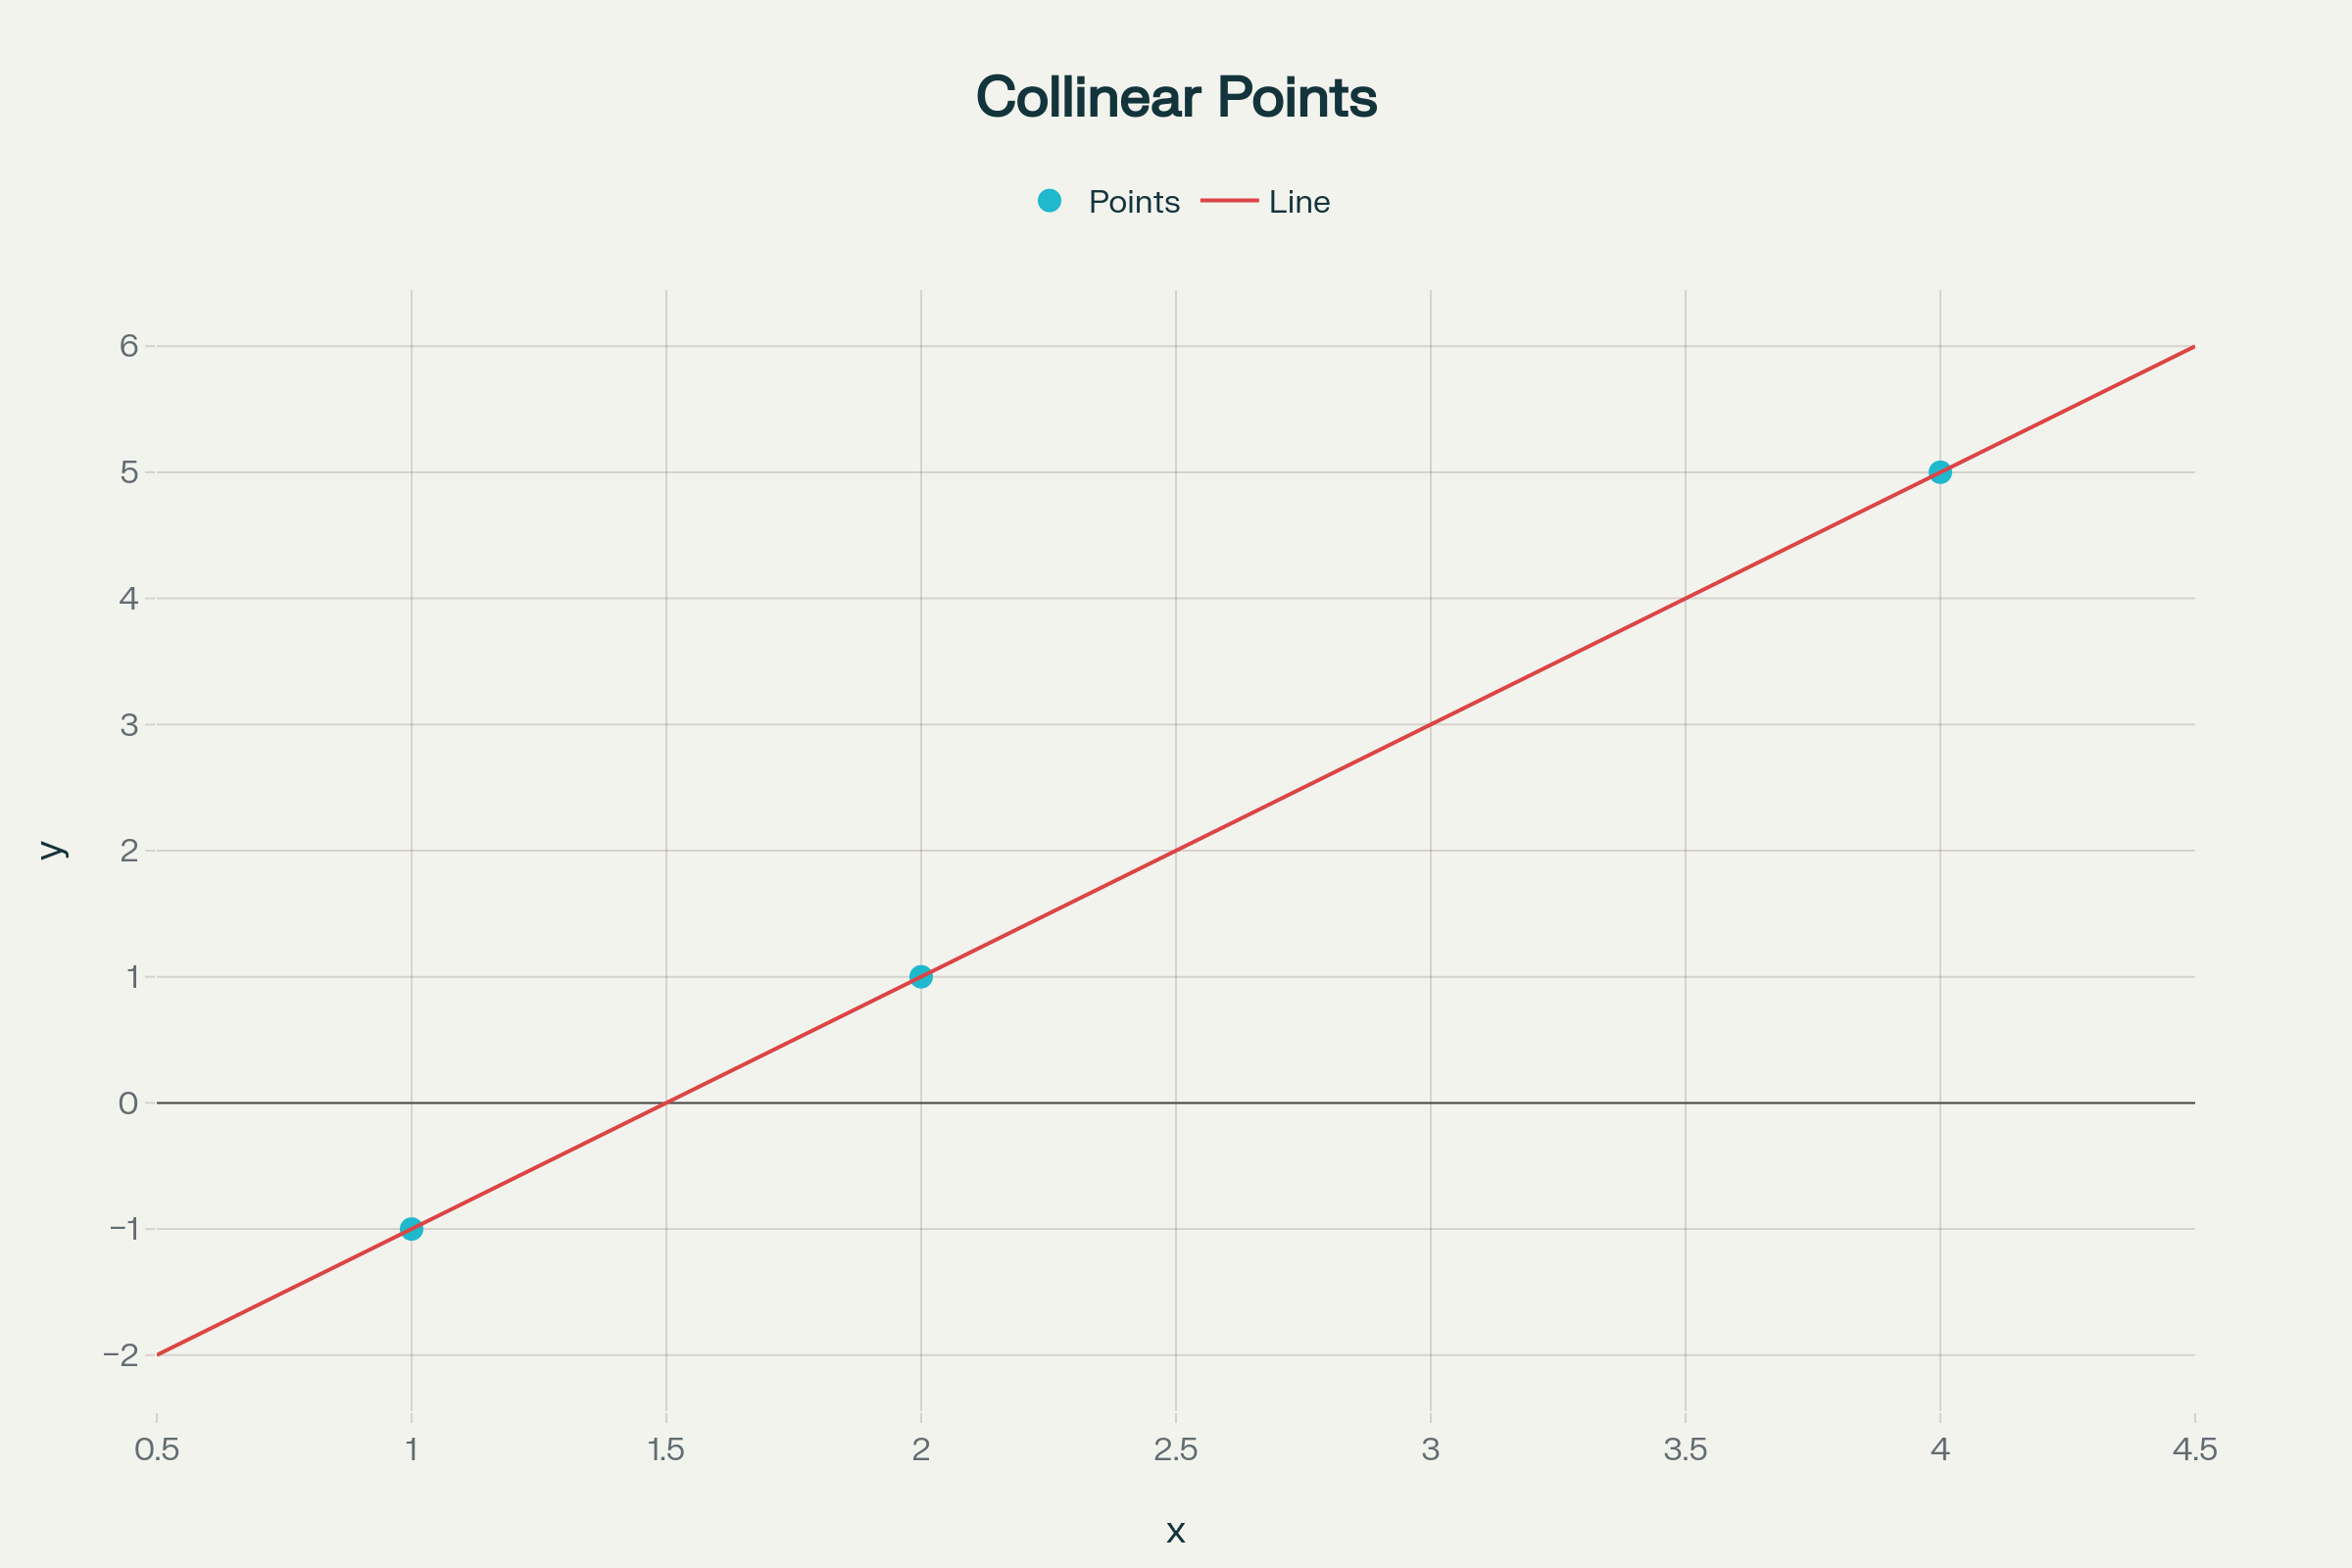
\includegraphics[width=0.8\columnwidth]{figs/fig.png}
    \caption{Collinearity}
    \label{fig:placeholder}
\end{figure}



\end{document}